\begin{figure}[h!]
\centering
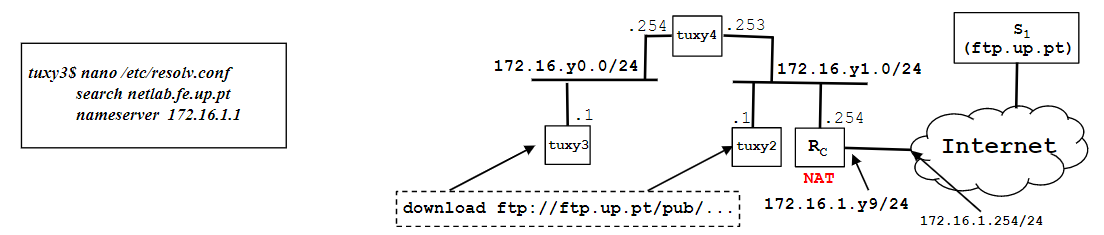
\includegraphics[scale=0.3]{imagens/Exp6.png}
\caption{Arquitetura da Sexta Experiência}
\label{fig:exp6}
\end{figure}

Os comandos usados para esta experiência podem ser encontrados no Anexo \ref{exp6_steps}.

Nesta experiência, a aplicação que elaborámos, foi compilada e executada. Durante a execução, são abertas duas conexões TCP. Uma, para a porta 21, utilizada para controlo, e outra, para uma porta a ser definida, utilizada para todo o transporte de dados. Para iniciar uma conexão TCP, em primeiro lugar, abre-se uma nova porta e, de seguida, é feita a conexão ao servidor usando essa mesma porta.

Foi feita a conexão no modo passivo, escolhido na criação
da aplicação, pois permite identificar a porta de retorno de maneira direta e, assim, iniciar uma nova ligação para a transferência binária.
Após a criação da nova ligação de dados é enviado o comando retr direcionado ao ficheiro a transferir. Recebe-se de seguida a FTP-DATA,  que indica o tamanho em bytes das tramas. Ao fim de cada trama é enviada uma mensagem ACK do cliente para o servidor para confirmar a receção dos dados. Ao chegar ao fim do ficheiro o servidor manda uma mensagem de sucesso com o código 226 para confirmar o fim da transferência do ficheiro. Todos estes passos descritos são visíveis nos logs da Figura \ref{fig:exp6_download_steps}.

O ARQ TCP é um mecanismo de controlo de erros na transmissão de dados onde pacotes de controlo ACK's são enviados pelo recetor, indicando a correta receção de uma trama de dados ou pacote. Os campos de maior relevância são o “sequence number field” e o “ACK number field”. O primeiro identifica o byte que representa o início da mensagem no pacote de dados, e o segundo identifica o número de sequência do próximo byte que o emissor do ACK espera receber em seguida.

Relativamente ao controlo de congestão, foi possível verificar que, durante a transmissão de dados, o recetor envia em cada mensagem ACK o tamanho da janela TCP que informa quantos bytes podem ser recebidos. Esta janela pode ficar cheia caso o cliente não esteja a ler dados de forma rápida o suficiente, sendo que quando isto acontece o recetor envia uma mensagem ACK com o bit window full ativo, fazendo com que o emissor pare de enviar dados temporariamente como se verifica nos logs da Figura \ref{fig:exp6_window_full}. Caso o emissor não respeite estas indicações, os bytes excedentes são descartados levando a retransmissões desnecessárias. Quando o receptor conclui a leitura de todos os bytes recebidos no pacote TCP este envia um TCP window update, indicando que está pronto para receber mais dados, esta mensagem é visível nos logs da Figura \ref{fig:exp6_logs_ACK_window_update}.

Teoricamente, ao aumentar o número de conexões TCP a largura de banda disponível para cada uma das conexões diminui, reduzindo consequentemente o throughput. Na prática, o gráfico que obtivemos relativo ao throughput (Figura \ref{fig:exp6_throughput_graph}) não foi de encontro ao esperado uma vez que não é notório no gráfico uma queda quando se iniciou o segundo download e consequentemente uma reposição do throughput quando o mesmo termina. Este resultado pode dever-se ao facto de o throughput se encontrar bastante abaixo da capacidade máxima de ligação fastethernet, fazendo com que não seja visível esta variação. Outra possibilidade é o facto de o tamanho dos pacotes lidos na nossa aplicação ser de apenas 1 byte, o que pode ter limitado a velocidade do download, estando o bottle neck no processo de leitura do ficheiro e não na largura de banda disponível na conexão TCP. Outros fatores podem ter influenciado este gráfico uma vez que se nota uma quebra perto do segundo 100, que nada tem a ver com os downloads efetuados por nós.

\begin{figure}[h!]
\centering
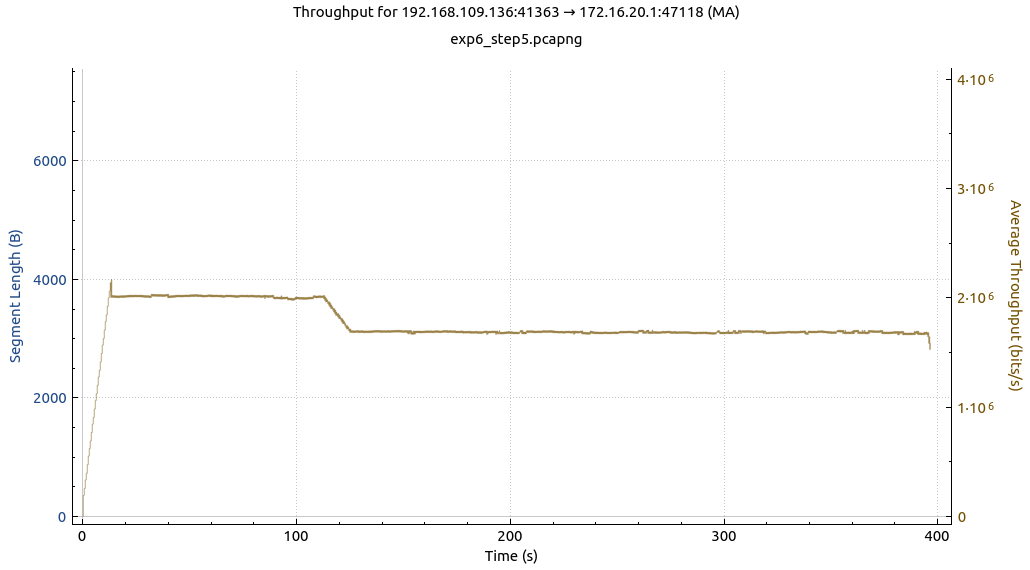
\includegraphics[scale=0.4]{imagens/exp6_throughput_graph.png}
\caption{Gráfico de throughput do download do ficheiro crab.mp4 na experiência 6}
\label{fig:exp6_throughput_graph}
\end{figure}